\documentclass{IEEEtran}

\usepackage{hyperref}
\usepackage{listings}
\usepackage{graphicx}
\graphicspath{{img/}}

\title{Florida Polytechnic University Campus-Wide Mesh Network}
\date{2015-07-17}
\author{Joseph Prine, John McCormack, Cody Madden, William Mathis, Ryan Integlia}

\begin{document}
\maketitle

\begin{abstract}
The Florida Polytechnic University embedded discovery platform will serve as an educational tool and research platform for students to develop network applications, technologies, and experiments.  As an educational tool, the network will provide students with hands-on experience in the development of sensor networks, as well as the exploration of software-defined radio and software-defined networks.  As a research platform, students will be able to develop applications and technologies related to gaming, social media, and security. As the project expands, the discovery platform will transition into a campus wide mesh network capable of larger scale testing. 
\end{abstract}
\begin{IEEEkeywords}
Software Defined Radio, ad-hoc network, mesh network, HCI, HMI
\end{IEEEkeywords}


\section{Introduction}
Wireless networks are quickly becoming a necessary infrastructure for the 21st century.  A reliable connection to the internet, or to specific intranets, is as critical as a connection to an electrical power grid for a growing number of applications.  Aside from the obvious network applications like communication and security, new ways to use networks are becoming more popular.  These applications include social networking, gaming, smart manufacturing, and smart devices like intelligent cars and wearable technology. Reliable, robust, and abundant wireless networks will allow a wide array of devices to communicate with each other, making the Internet of Things possible.
\section{Network Architecture}
The Florida Polytechnic University Mesh Testbed essentially takes the form of a mobile ad-hoc network, or MANET.  The wireless multi-hop communication of the mesh network, communicating with the world wide web via multiple gateway nodes, forms a flexible network for communication. The network is currently made up of several small, battery operated wireless routers running OpenWRT. OpenWRT is an open source, freely available operating system with a large community of developers. Batman-adv is used as the mesh routing protocol. Two separate images have been built to create the appropriate infrastructure. One set act as gateways to traditional internet infrastructure. The others relay data packets to one another using the batman-adv protocol. Physically, the nodes are the same. This means with a change in software any one node could act as the role of another. The nodes are all able to be updated remotely so a change in software does not require a person to manually go to each node and change settings. 

\begin{figure*}
	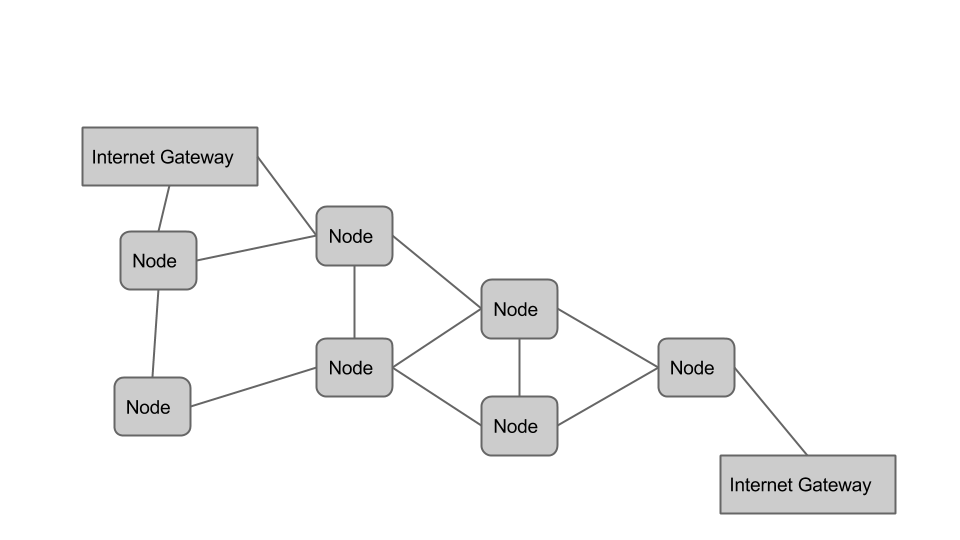
\includegraphics[width=\textwidth]{nodearchitecture}
	\caption{A brief overview of the mesh architecture}
\end{figure*}
\section{Data Collection}
The goal of the mesh network is to implement a distributed, wireless, data collection platform. Currently, Raspberry Pi microcomputers are connected to various sensors. The Raspberry Pi’s can then utilize the mesh network to send the data to a central server for storage and processing. Alternatively, preprocessing can be handled by the raspberry pi, and only the needed data can be sent over the network. The Raspberry Pi is an open source, low power, microcomputer that allows us to collect more data than would be possible on a simple microcontroller. However, because batman-adv presents the network transparently to the computer, it would be possible to switch to a microcontroller without any change to the rest of the infrastructure. This would allow for data collection over a longer period of time, with less resources. The sensor data is collected using a program written in Node.js. The data is then sent out over the mesh using the socket.io library for Node.js. 

\subsection{Data Visualization}
    Pure data is rarely helpful on its own. Being able to interpret the data is what is useful and interesting. We are working towards creating a visualization system within the Unity game engine. Unity is not open source, but it is freely available and features the ability to compile software for nearly every major computer, mobile, and video game platform. We currently have a demonstration that allows for a user to interact with a node, and see a reaction within the Unity environment. The user can also interact with a virtual representation of the node in Unity to cause a change on the real node. This was tested and found to work over the mesh network. The Raspberry Pi software was developed in Python using the Flask framework. Unity and the Raspberry Pi interact with a PostgreSQL database. When a new node is activated on the mesh, the raspberry pi will update the database, giving the database its IP Address. Unity will then create a new node whenever it sees a change in the database.  The Raspberry Pi’s can then update the PostgreSQL database with changes to the state of the push button or other sensors. Unity will then respond appropriately and update the information about each sensor node. As the available tools for data collection increases, we will be able to increase the available options for data visualization. 
\section{Future Work}

\subsection{Data Interaction and Human Machine Interfaces}
In order to make the interaction with the data more natural and innovative, we will seek to employ various human machine interfaces  (HMI) with the Unity system. We have begun to experiment with the Myo Armband, Neurosky EEG device, Leap Motion Plus, and 2D Lidar systems. Each of these tools presents a unique human computer interaction (HCI) method that could allow a user to go beyond a normal mouse and keyboard setup. These systems could also be paired with an Oculus Rift virtual reality headset to give the user the ability to entirely immerse themselves in the data visualization environment.  As a data set grows, it becomes more and more difficult to present it to a user in a way that a traditional 2D computer screen and mouse can be useful for interacting with. We seek to use these emerging tools to remove the barriers normally associated with data interaction. 

\subsection{Software Defined Radio and Cognitive Networks}

To increase the security, network reliability, and scalability of the platform, we will look to use software defined radios to create a cognitive mesh network. Software defined radios abstract most of the components of a wireless transceiver into software. This allows them to act as many different types of radios over a wide range of frequencies. By scanning the adjacent area for open frequencies, the mesh network could be designed to hop from frequency to frequency. This allows the radios to always communicate in a free band without interrupting any other transmissions. We are currently exploring the use of GNU Radio for cognitive networks and have successfully run some basic SDR tests using this free and open source software tool. We would like to integrate the frequency hopping into the Unity game engine so that the visualization of the network topology will include a depiction of what frequency each node is broadcasting at. 

\subsection{Unity Gamification for Testing}

In order to properly test the mesh network, we will need a way to incentivise users to use the mesh.  We will use the Unity game platform to create different augmented reality video games that will reward users for interacting with the mesh. One proposed project, called “mesh trader”, chooses one node at random, and points are awarded when a user reaches and connects to the node. This way, we will cause a surge of data to be transferred over one node to see how the network reacts. After initial tests using Humans with mobile phones, we would like to implement a similar game using UAVs. This will put a tremendous strain on the mesh as the drones are capable of transmitting telemetry data and video and will need to constantly be receiving commands from a user as the game is played. 

\subsection{Data Visualization}
We will seek to expand upon our current system for visualization. Using Unity, we would like to create a much more involved data visualization system capable of displaying network, sensor, and interaction data over the mesh network. As work progresses, we will seek to incorporate new and innovative display methods such as the Oculus Rift Virtual Reality headset and possibly other virtual and augmented reality devices. 

\subsection{Adaptability and Mobility}
One of the most exciting applications of the mesh network is for the distributed control of robots including Unmanned Aerial Vehicles (UAVs) and Unmanned Submersible Vehicles (USVs). Research has begun at other universities into controlling UAVs using this type of network, however almost all of it is in the simulation level. Florida Polytechnic could become the leader in this quickly emerging field. A base station could be established within the VTC or a similar lab space on campus. Once connected to the node, commands could be sent to the robot, while live data is returned to the base station for processing. Color changing smart lighting on the node could change to indicate which node is currently connected to the UAV. While not strictly necessary, this would allow students to see a visualization of packets flowing through the mesh. More importantly, these robots could allow the shape of the network to change with the needs and capacity of the system. If a particular node breaks, or if one node becomes overcrowded, a robot could physically move another node into proximity of the area that needs it. 

This concept could be expanded to swarm robotics. A huge portion of the research involved in swarm robotics is on intraswarm communication. In order for the group to function, appropriate information must be able to flow through the swarm. The mesh nodes would allow this data to be transported over a wide area from robot to robot. Human Swarm Interaction is also an emerging field. The VTC could be given proper equipment to allow work to be done in this field. A system involving an oculus rift and a joystick or gamepad could be used to create a simulated cockpit. Users could then watch the gross movement of the swarm on projectors in the VTC. These projectors could show where on a map the robots are as well as stream live video feed from the group. Pilots could then use the rift and joystick to control specific robots.

\end{document}
